%!TEX root = thesis.tex
\chapter{Body Part Detection}
\label{ch:bodyparts}


\section{Finding hands}
To do hand pose estimation of a person in a image his or her hands need to be localized in the image first. Since hands can have different shapes, different orientations, specific color profiles and shapes per person this is a very difficult task. One way to localize the hands is by searching for skin like colors in an image given that this color profile is known. A generic skin model has been build for this purpose\cite{Jones99statisticalcolor}, but using these values for searching in a image is quite sencetive for error. Skin color can vary dramatically because of lightning conditions but also the cameras properties can color a image. It would be much better to have a way where the skin color the hands could be extracted from the target image itself. This can be done by detecting the subjects face in an image.

\section{Face detection - Haar classifier}
Finding faces in a image is a rather well solved problem. Faces are easy to detect, since it has easy to detect features like eyes, eyebrows, a mouth and nose. When comparing different faces, these features are - with a small variation - on the same distance and orientation. Also people don't tilt their head often, or not more than a couple degrees.

Face detection can be done in a fast and robust way using a haar classifier, a boosted rejection cascade that is trained with Haar-like wavelet.
 features\cite{Lienhart02anextended}. Haar wavelets, histogram building.


\section{Color space conversion}
Usually pixel values of a image are stored in the Red, Green Blue (RGB) format. Advantages can be gained by converting this color space into an other so, for example thresholding on one channel or even leaving on channel out gets a different meaning. One particular color space that is interesting for this application is the Hue Saturation Value (HSV) color space. HSV space separates out Hue (color) from Saturation (how concentrated the color is) and from Value (brightness). 

\begin{figure}[htbp]
	\center
	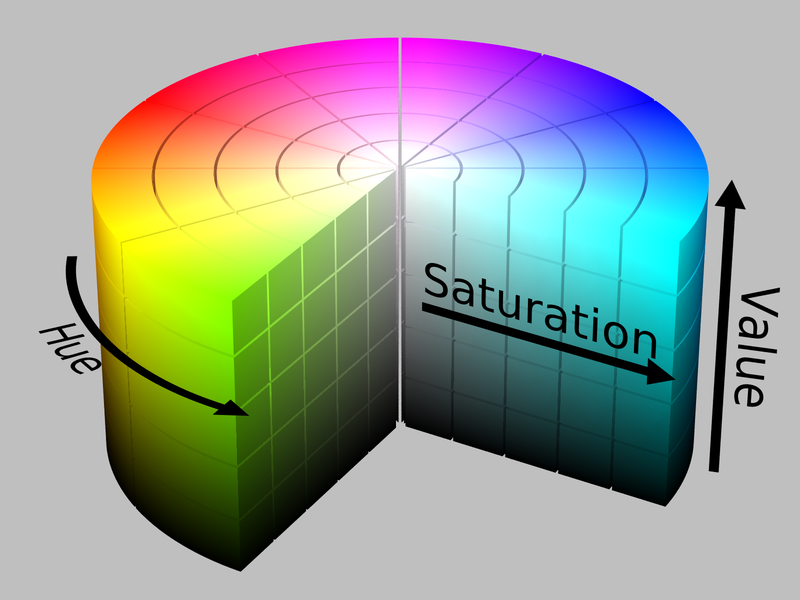
\includegraphics[width=0.4\linewidth]{figures/hsv.png}
	\caption{The Hue, Saturation, Value color space}
	\label{fig:hsv}
\end{figure}

The color models are created by taking 2D histograms from the H (hue) channel in HSV space.





The RGB color space is transformed into the HSI color space using the following equations:


\begin{eqnarray*}
  V & \leftarrow & \max(R,G,B) \\
  S & \leftarrow & \left\{
  \begin{array}{l l}
    \frac{V-\min(R, G, B)}{V} & \quad \text{if $V \neq 0$} \\
    0 						  & \quad \text{otherwise} \\
  \end{array} \right.\\
  H & \leftarrow & \left\{
  \begin{array}{l l}
    60(G - B)/S     & \quad \text{if $V \eq R$} \\
    120 + 60(B-R)/S & \quad \text{if $V \eq G$} \\
    240 + 60(R-G)/S & \quad \text{if V \eq B} \\
  \end{array} \right.\\
\end{eqnarray*}
  



\section{Skin color histogram}
When a face is found a color model for the subjects skin can be created. this is done by constructing a 2 dimensional histogram with the Hue and Saturation values. A histogram is a n-dimensional matrix, where every dimension is devided into bins. A bin corresponds to a range of values for each dimension. A histogram is constructed by creating an empty matrix. For every pixel in the image the coresponding bin is ditermined, and the value of the bin is increased by one. When all pixels are evaluated, the histogram is normalized - all values are devided by the sum. This way when all values are added together, the sum wil be equal to 1. This makes the histogram independent of the image size. There are not really optimal values for the number of bins, around 30 for each is good.\marginpar{WHY} The resulting histogram is a model for the faceskin hue and saturation in the original image.

\begin{figure}[htbp]
	\center
	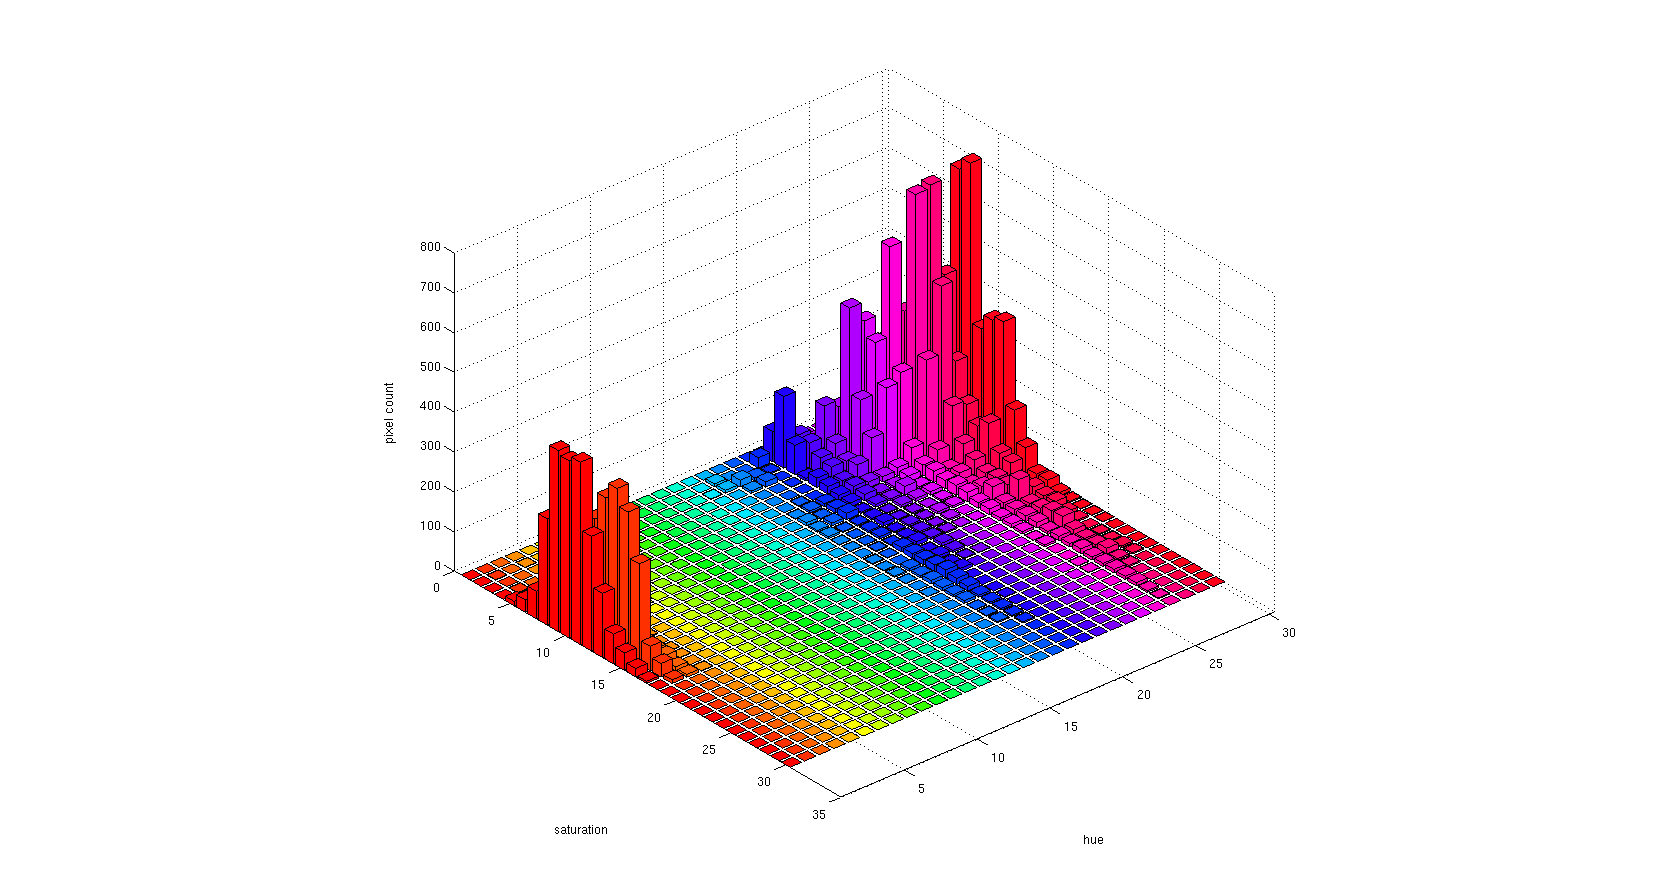
\includegraphics[width=0.8\linewidth]{figures/face_hist.png}
	\caption{Histogram of a face}
	\label{fig:face_hsv}
\end{figure}

\section{Back projection}
A back projection is the combination of a image a histogram. The result is a new single channel image. All pixels in the input image are iterated and the corresponding bins are looked up in the histogram. The pixel in the same position in the new image is replaced with the value from the histogram. If the histogram is a skin color histogram, the resulting image will have high values for pixels that are skin-like pixels, and low values for other pixels. These values can be seen as skin probability.
A backprojection is the process of replacing all original pixel values with the corresponding histogram bin value. This will result in a single channel probabalistic image, where each pixel corresponds to the probability being a face like pixel. Pixels with a face skin like color will have a high value, other pixels, for example background pixels will have a low value.

\section{Threshold}
To binary label every pixel to be skin color or not, we need to define a way of doing this automatically. The easiest way to accomplish this is by defining a threshold. All pixel values below a certain threshold are replaced with false or 0, all above this threshold will be replaced with true or 1. This results in a binary image with labels for (non) skin pixels. This method introduces one parameter - the threshold for going from the probabilistic domain to the binary domain.

\section{morphological operation - closing}
untill now each pixel has been processed independently, and the information in surrounding pixels is ignored. In natural images, strong gradients are rare. Pixel values close to each other in the image are usually also close to each other in the HSV domain. This is also true for skin like pixels and non skin like pixels. In other words said; if a pixel is a skin pixel, then the neighbours are probably also skin pixels and the opposite. To encorporate this implicit information the morhological operations can be used.

There are 2 basic morhological operations which can be used seperatedly or in sequence - the erode operation and the dilate operation which are strongly related. The input for the operations is a binary image and a kernel. A kernel can be any 2D binary matrix, but usually an elliptic shape is used. When performing the erode operation on a input image $A$ with kernel $K$, all false pixels in $A$ are itterated. In every iteration the surrounding pixels of the current itterated pixel are replaced with the false values in $K$, with the center of $K$ as relative point of the current iteration point. The result is that the binary true shapes in $A$ are 'eroded'. This is the same for dilation, but the opposite way. One could also say that in the case of dilation the background, or false pixels are 'eroded'. 

The closing of A by B is obtained by the dilation of A by B, followed by erosion of the resulting structure by B:
Back projection, morphological transformations

ALSO TELL SOMETHING ABOUT NOISE 

\section{Pixel grouping, contour extraction}
To be able to say something usefull about groups of pixels, one need to know which pixels belong together. This can be done by contour extraction. Contour extraction is performed by labeling all touching pixels together.

\section{Blob labeling}
Heuristics for blob labeling

\section{Blob label stabilization}
Kalman filter (prediction) and template search

\section{Discussion}
Ignoring the Value channel in the HSV color space to make the system invariant for lighting intensity changes assumes that the light source is pure white - a saturation of zero. In reality this is never the case, since creating artificial light that is pure white is difficult to accomplish, if not impossible.

A parameterless method of going from the probabilistic domain to the binary domain is adaptive thresholding.

The face detection is one of the most expensive operations in the processing chain. Since in a single shot movie usually a face doesn't move fast, a number of frames can be skipped which will free more computational time for other operations.

\begin{figure}[htbp]
\begin{center}
\subfloat[input frame]{\label{fig:pipe_input}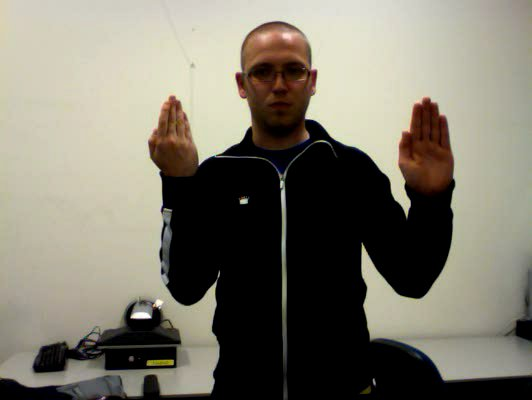
\includegraphics[width=0.45\linewidth]{figures/pipeline/input3.jpg}}
\hspace{0.03\linewidth}
\subfloat[face detection]{\label{fig:pipe_detected}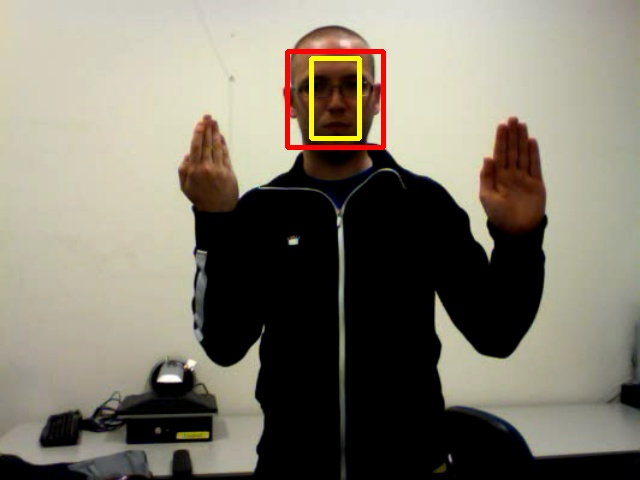
\includegraphics[width=0.45\linewidth]{figures/pipeline/detected.jpg}}
\hspace{0.03\linewidth}
\subfloat[Face color histogram]{\label{fig:pipe_hist}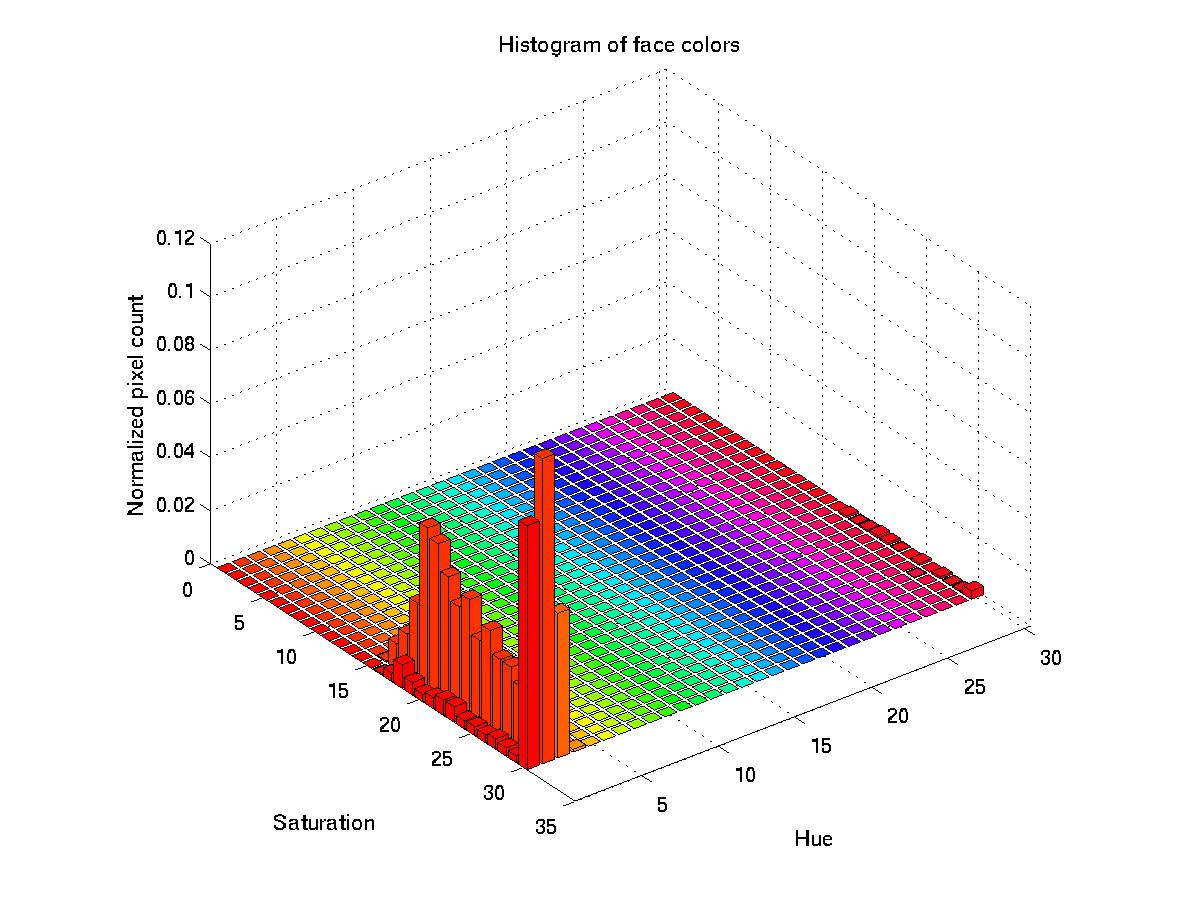
\includegraphics[width=0.45\linewidth]{figures/pipeline/histobar.jpg}}
\hspace{0.03\linewidth}
\subfloat[Backprojection]{\label{fig:pipe_bp}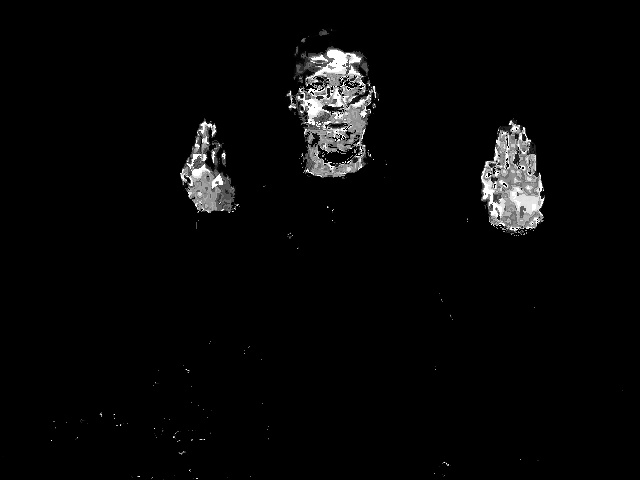
\includegraphics[width=0.45\linewidth]{figures/pipeline/backproject.jpg}}
\hspace{0.03\linewidth}
\subfloat[Gaussian smooth]{\label{fig:pipe_blur}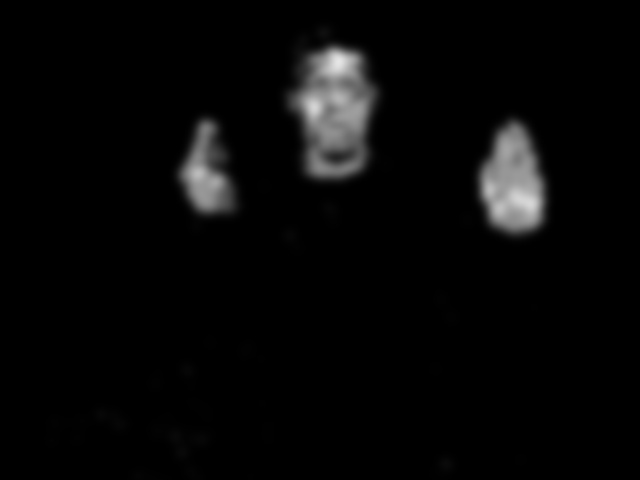
\includegraphics[width=0.45\linewidth]{figures/pipeline/blurred.jpg}}
\hspace{0.03\linewidth}
\subfloat[Thresholded binary image]{\label{fig:pipe_th}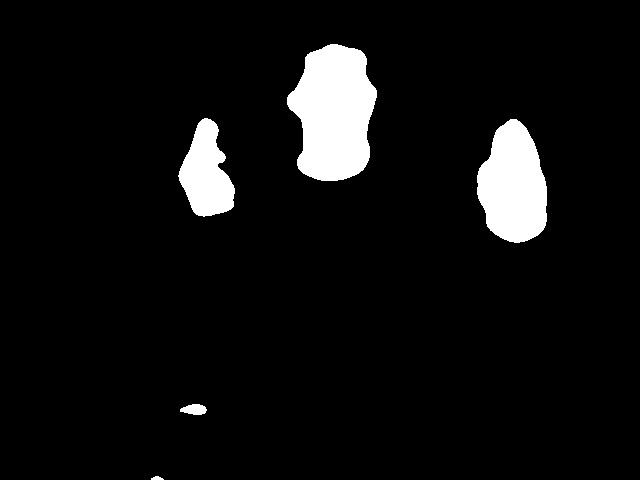
\includegraphics[width=0.45\linewidth]{figures/pipeline/thresholded.jpg}}
\hspace{0.03\linewidth}
\subfloat[Morpholoical close]{\label{fig:pipe_close}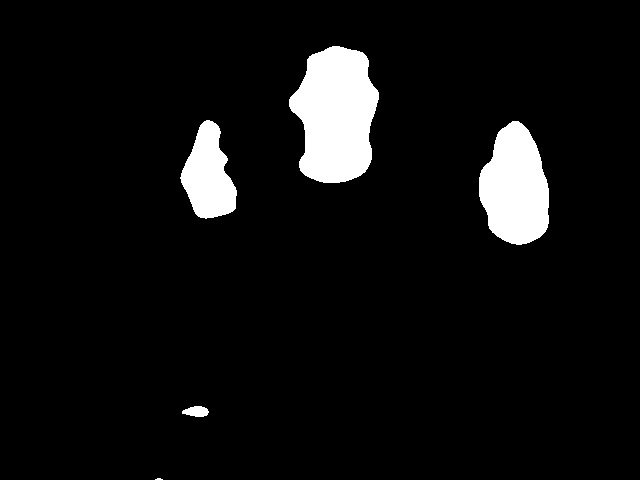
\includegraphics[width=0.45\linewidth]{figures/pipeline/closed.jpg}}
\hspace{0.03\linewidth}
\subfloat[Blob labeling]{\label{fig:pipe_cont}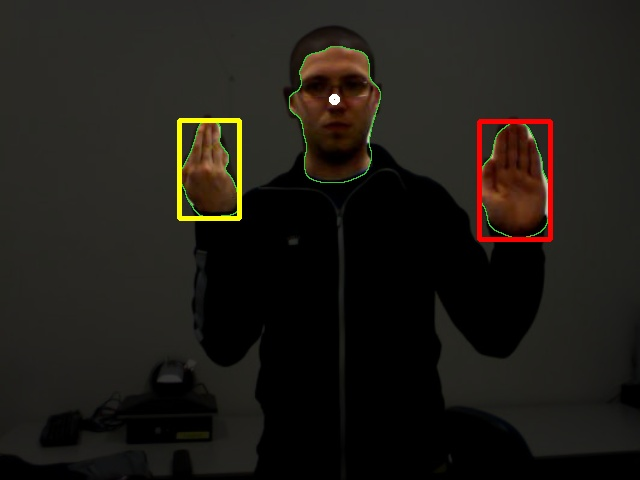
\includegraphics[width=0.45\linewidth]{figures/pipeline/contours.jpg}}
\end{center}
\caption{The hand detection pipeline}
\label{fig:pipeline}
\end{figure}

